
\section{Related work}
% Time series forecasting is a topic that have been around since at least the 80's and is a subject that can be applied in various domain like our energy consumption but also trading, medicines which mean that a lot reasearch has been done. 
% \par
% Since the 80's a lot informatic has change, research over this subject has also evolved with the new technics found in the rest of the AI research fies I.E that it beeggan with signal processing method and the it evolved to more machine learning process. It also seen a lot of evolution in machine learning starting with random forest, then having MLP (multi layer perceptron), CNN (convolutionnal neural network), RNN (recurant neural network) and finaly transformers. So this mean that we have lot of choice in our model selection\cite{De_Gooijer2006-mi, Hahn2023-rc}.
% \par
% Per stated in the introduction we are going to use different class of model. For each model that we will be using we are going to introduce theoricaly the model and what we expect from it.

% \par
% One of the oldest modal than we can find that has been used a lot is ARIMA which stand for \emph{autoregressive integrated moving average}. This method is based on signal processing and try to mitigate 3 principle toegether : 
% \begin{itemize}
%     \item AutoRegressive : the part that will look at past data
%     \item Integrated : differentiate the serie to make the distribution remain stationnary which elimanted seasonal effect.
%     \item Moving Average : extract relationship between data and residual error. Which is usefull to track short-term changes.
% \end{itemize}
% To find all parameter of this method, it is pretty common to use \emph{Box-Jenkis} method\cite{Shumway2017-kk} but other method also exist and nowadays python libraries implement method to find good parameters.
% \par
% ARIMA model is not perfect so there exist a lot variant that comes to correct a problem. By example SARIMA which allow ARIMA model to be used on stationary time series. \cite{Valipour2015-sv} Staionarity is the property of the dataset to have a constant mean, auto-correlation and variance.

Time series forecasting has been an active area of research since at least the 1980s and has found applications in a wide range of domains, including energy consumption, financial markets, and healthcare. Due to its practical importance, the field has attracted substantial research attention over the past decades.

\par
Since the 1980s, major advances in computing power and data availability have significantly influenced the evolution of time series forecasting methods. Early approaches were primarily based on signal processing and statistical modeling techniques. %Over time, these methods have been progressively complemented—and in some cases replaced—by machine learning and, more recently, deep learning approaches. This evolution mirrors broader developments in artificial intelligence research.

\par
Machine learning methods for time series forecasting have evolved from classical algorithms such as random forests to neural network-based models, including multilayer perceptrons (MLP), convolutional neural networks (CNN), recurrent neural networks (RNN), and, more recently, transformer-based architectures. As a result, a wide variety of models are now available, each with distinct assumptions, strengths, and limitations \cite{De_Gooijer2006-mi, Hahn2023-rc}.

% \par
% As stated in the introduction, this work considers several classes of forecasting models. For each model, we provide a theoretical overview and discuss the expected behavior and performance characteristics. %REVENIR

\par
One of the earliest and most widely used statistical models for time series forecasting is the ARIMA model, which stands for \emph{AutoRegressive Integrated Moving Average}. ARIMA models are rooted in classical time series analysis and are designed to capture temporal dependencies through three main components:
\begin{itemize}
    \item Autoregressive (AR): models the dependence between an observation and a number of its past values.
    \item Integrated (I): applies differencing to the time series in order to achieve stationarity.
    \item Moving Average (MA): models the dependence between an observation and past forecast errors, which is particularly useful for capturing short-term fluctuations.
\end{itemize}

\par
The parameters of an ARIMA model are traditionally identified using the Box--Jenkins methodology \cite{Shumway2017-kk}, although alternative approaches exist. Modern statistical software libraries provide automated procedures for parameter selection.

\par
Despite its effectiveness, the ARIMA model has limitations, particularly when dealing with seasonal patterns. Several extensions have been proposed to address these issues, such as the Seasonal ARIMA (SARIMA) model \cite{Valipour2015-sv}, which explicitly incorporates seasonal components.% Stationarity, in this context, refers to the property of a time series whose statistical characteristics—such as mean, variance, and autocorrelation—remain constant over time.




% \par
% In the deep learning model, there is a lot of model that can be used. Some are bette suited to tackel prediction of timeserie like familiy recusive neural network (RNN)  or the transformer model familiy. 
% \par

% The idea behing the family of RNN is a model that for each timestamp will take a value (or vector) as input. With this, it will update his internal vector that represent the memory of the model. With this memory he can output a vector to predict the next element. By this design it could theoricaly handeld infine long sequence which is interessting\cite{Schmidt2019-kw}. The Figure~(\ref{fig:rnnarchitecture}) show the architecture of this model.

% \begin{figure}[H]
% \centering
% 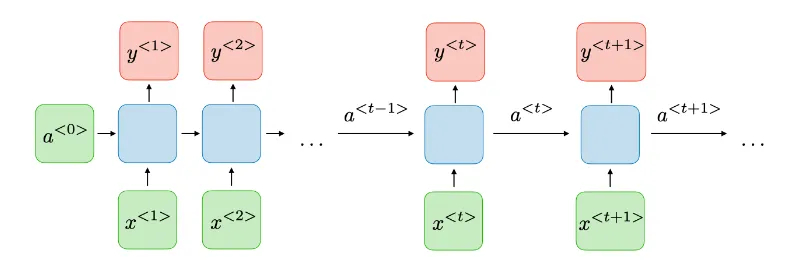
\includegraphics[width=0.80\textwidth]{images/rnn_architecture.jpg}
% \caption{RNN Architecture}
% \label{fig:rnnarchitecture}
% \end{figure}


% In the family of RNN, there is also the model LSTM (Long Short-Term Memory). The there existe different version and the version a bit more advanced is LSTM for long short term memory. This variant arise to counter some limitation of RNN such as vanishing gradient that make it hard to train RNN models on very long series so making hard for to model long term relation ship. Both of this model has still the bottle neck to only have one internal representation. 
% \par


% In the other hand the transformer family that us the concept of attention to avoid unic interal representation that is bottlenecking RNN family. It was at the basis developped for NPL\cite{Vaswani2017-jv}. But a sentence can be represented in a time serie where at each step we have a word. So this principe can easily be reused and has been reused to trackle time series forecasting. 

% \par
% The attention (or self-attention in our case) is a mecanism that is capable of dynamicaly assign importance weight (or attention weight) to different element in the input series. Which completely overcome the bottle neck of having only one representation of memory.
% \par
% By looking at state of the art method used in currently libraries. They claim that it surpass everything that was known\cite{Zerveas2021-ff}. They also talk that those new implementation can be trained with fewer data so we should be able to train the model. 

Among deep learning approaches, several model architectures can be applied to time series forecasting. Some families of models are particularly well suited for sequential data, including recurrent neural networks (RNNs) and transformer-based architectures.

\par
The core idea behind the RNN family is to process sequential data by iteratively updating an internal hidden state. At each time step, the model receives an input value (or vector), which is used together with the previous hidden state to update the internal representation of the sequence. This hidden state serves as a form of memory and can be used to generate an output, such as a prediction of the next time step. Due to this recursive structure, RNNs are, in theory, capable of handling sequences of arbitrary length \cite{Schmidt2019-kw}. Figure~\ref{fig:rnnarchitecture} illustrates the general concept of an RNN.

\begin{figure}[H]
\centering
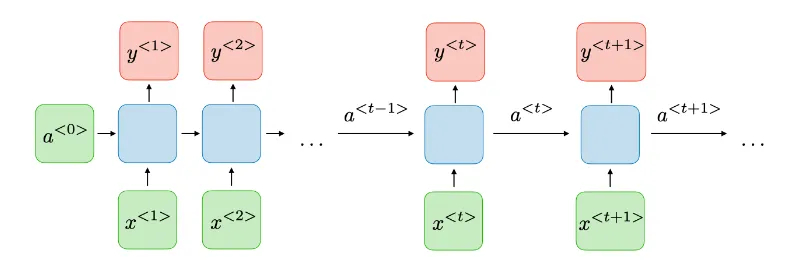
\includegraphics[width=0.80\textwidth]{images/rnn_architecture.jpg}
\caption{Recurrent Neural Network (RNN) concept where $x$ represent the input, $a$ the hidden state and $y$ the output value}
\label{fig:rnnarchitecture}
\end{figure}

\par
Within the RNN family, Long Short-Term Memory (LSTM) networks represent an important extension. Several variants of LSTM architectures exist, all designed to address key limitations of standard RNNs. In particular, LSTMs mitigate the vanishing gradient problem, which makes it difficult for vanilla RNNs to learn long-term dependencies in long sequences. By introducing gating mechanisms, LSTMs are better suited to modeling long-range temporal relationships. However, both RNNs and LSTMs remain constrained by the use of a single hidden-state representation, which can act as a bottleneck when modeling complex dependencies.\cite{Waqas2024-xj}

\par
In contrast, transformer-based models rely on the attention mechanism to overcome this limitation. Originally developed for natural language processing tasks \cite{Vaswani2017-jv}, transformers do not rely on recurrent computations. Instead, they process sequences by allowing each element to directly attend to all other elements in the sequence. Since a sentence can be viewed as a time-ordered sequence of tokens, this framework naturally extends to time series forecasting and has been widely adopted in this context.

\par
The attention mechanism, and more specifically self-attention, dynamically assigns importance weights to different elements of the input sequence. This enables the model to capture both short-term and long-term dependencies without relying on a single compressed memory representation, thereby alleviating the bottleneck inherent in RNN-based models.

\par
Recent state-of-the-art transformer-based models for time series forecasting have demonstrated strong empirical performance and outperform traditional statistical and recurrent neural network approaches \cite{Zerveas2021-ff}. Additionally, they report improved data efficiency compared to earlier deep learning models, making these architectures particularly attractive in practical forecasting settings.